\subsection{Wanderman Piran}
\label{ssec:WP}
Wanderman and Piran \cite{WP} extracted a GRB distribution in redshift and
luminosity using GRB data up to 2009 applying detection efficiencies for
both the detection in $\gamma$- rays and a following determination of the host
redshift, i.e., the redshift of the GRB. 

The differential co-moving rate of bursts (fig. \ref{fig:GRB_rate_density}) at a
redshift $z$ is
\begin{equation}
 R(z) = \frac{R_{\text{GRB}}(z)}{(1+z)} \frac{dV(z)}{dz}
 \label{eq:Rz}
\end{equation}
$dV(z)/dz$ is the differential co-moving shell volume 
and the factor $(1+z)^{-1}$ reflects the cosmological time dilation.
$R_{\text{GRB}}$ is fitted to data with the result (Fig \ref{fig:RGRB})
\begin{equation}
\label{eq:R_z}
    R_{\text{GRB}}(z) = \begin{cases}
                        \rho_0 \cdot (1 + z)^{n_1} & z \leq z_1 \\
			 \rho_0 \cdot (1 + z_1)^{n_1 - n_2}(1 + z)^{n_2} & z >
z_1
                        \end{cases}
\end{equation}
with
$n_1= 2.07$, $n_2=-1.36$, $z_1=3.11$ and the local rate $\rho_0=1.25
\text{Gpc}^{-3} \text{yr}^{-1}$.

% 1.25 \cdot 10^{-9} \cdot \text{Mpc}^{-3} \cdot \text{yr}^{-1}$

\begin{figure}[h]
\centering
 \captionsetup{width=.9\textwidth}
%  \captionsetup{margin=0pt}
\subfloat[Derived RGRB function (WP)\label{fig:RGRB}]{%
 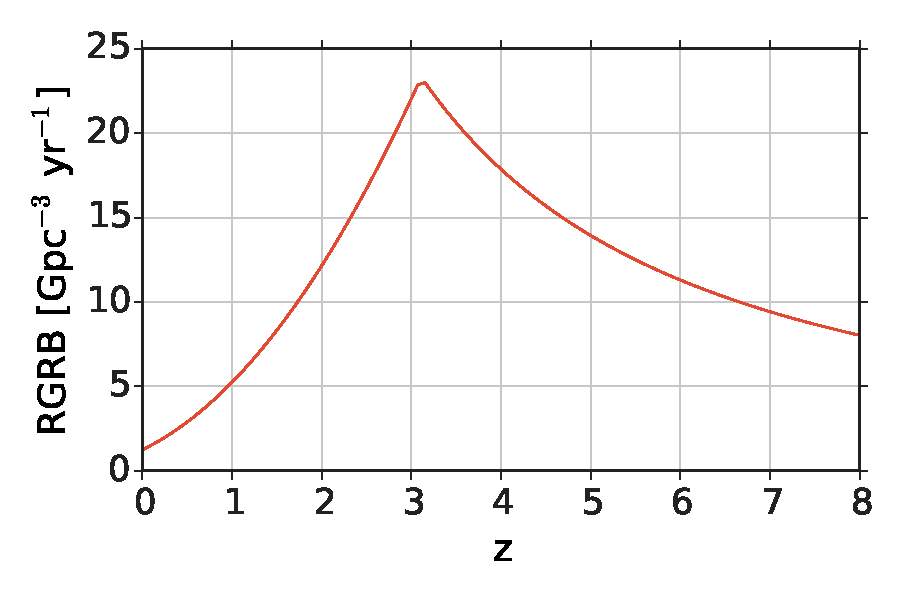
\includegraphics[width=0.45\textwidth]{fig/RGRB_WP.pdf}}
 \subfloat[Differential co-moving rate\label{fig:GRB_rate_density}]{%
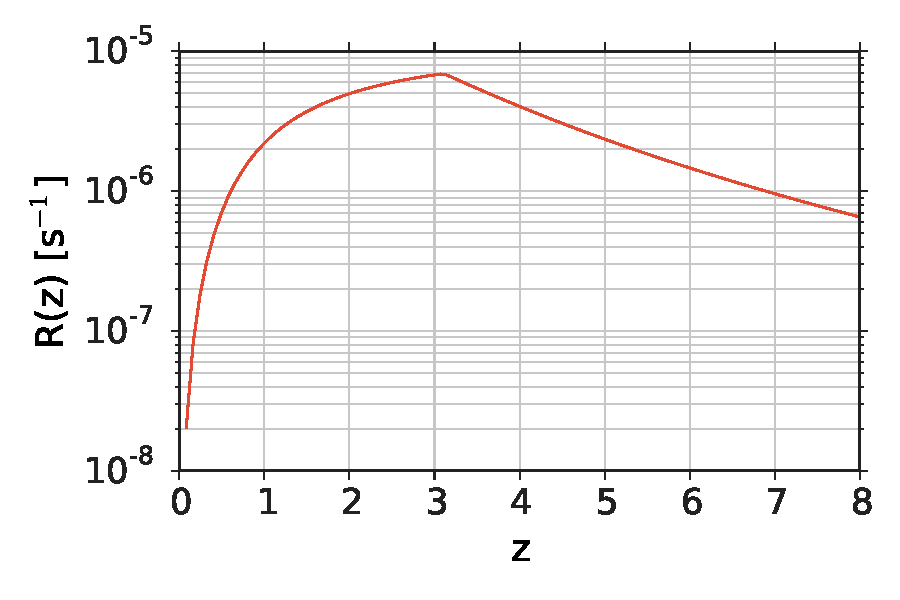
\includegraphics[width=0.45\textwidth]{fig/Rz_WP.pdf}}
\caption{The distribution of GRBs over the redshift displaying the derived RGRB 
function and the differential co-moving rate.}
\end{figure}




The peak $\gamma$-luminosity at the source
$L_{\text{Peak}}$ (Fig. \ref{fig:Lpeak})  is determined to follow
\begin{equation}
\label{eq:Phi_L}
 \Phi(L_{\text{Peak}}) = \begin{cases}
      \left(\frac{L}{L_{*}} \right)^{-\alpha} &  L < L_{*} \\
      \left(\frac{L}{L_{*}} \right)^{-\beta}  &  L > L_{*}
     \end{cases}
\end{equation}
in which $\text{log}_{10}L_{*}=52.53 \text{ erg / s}$ is the break luminosity
and $\alpha=0.17$ and $\beta=1.44$ are the spectral indices (Table
\ref{tab:grb_model_params}).
No redshift evolution of the luminosity is assumed.
\begin{figure}[h]
% \begin{minipage}{\textwidth}
 \captionsetup{width=.6\textwidth}
 \centering
%  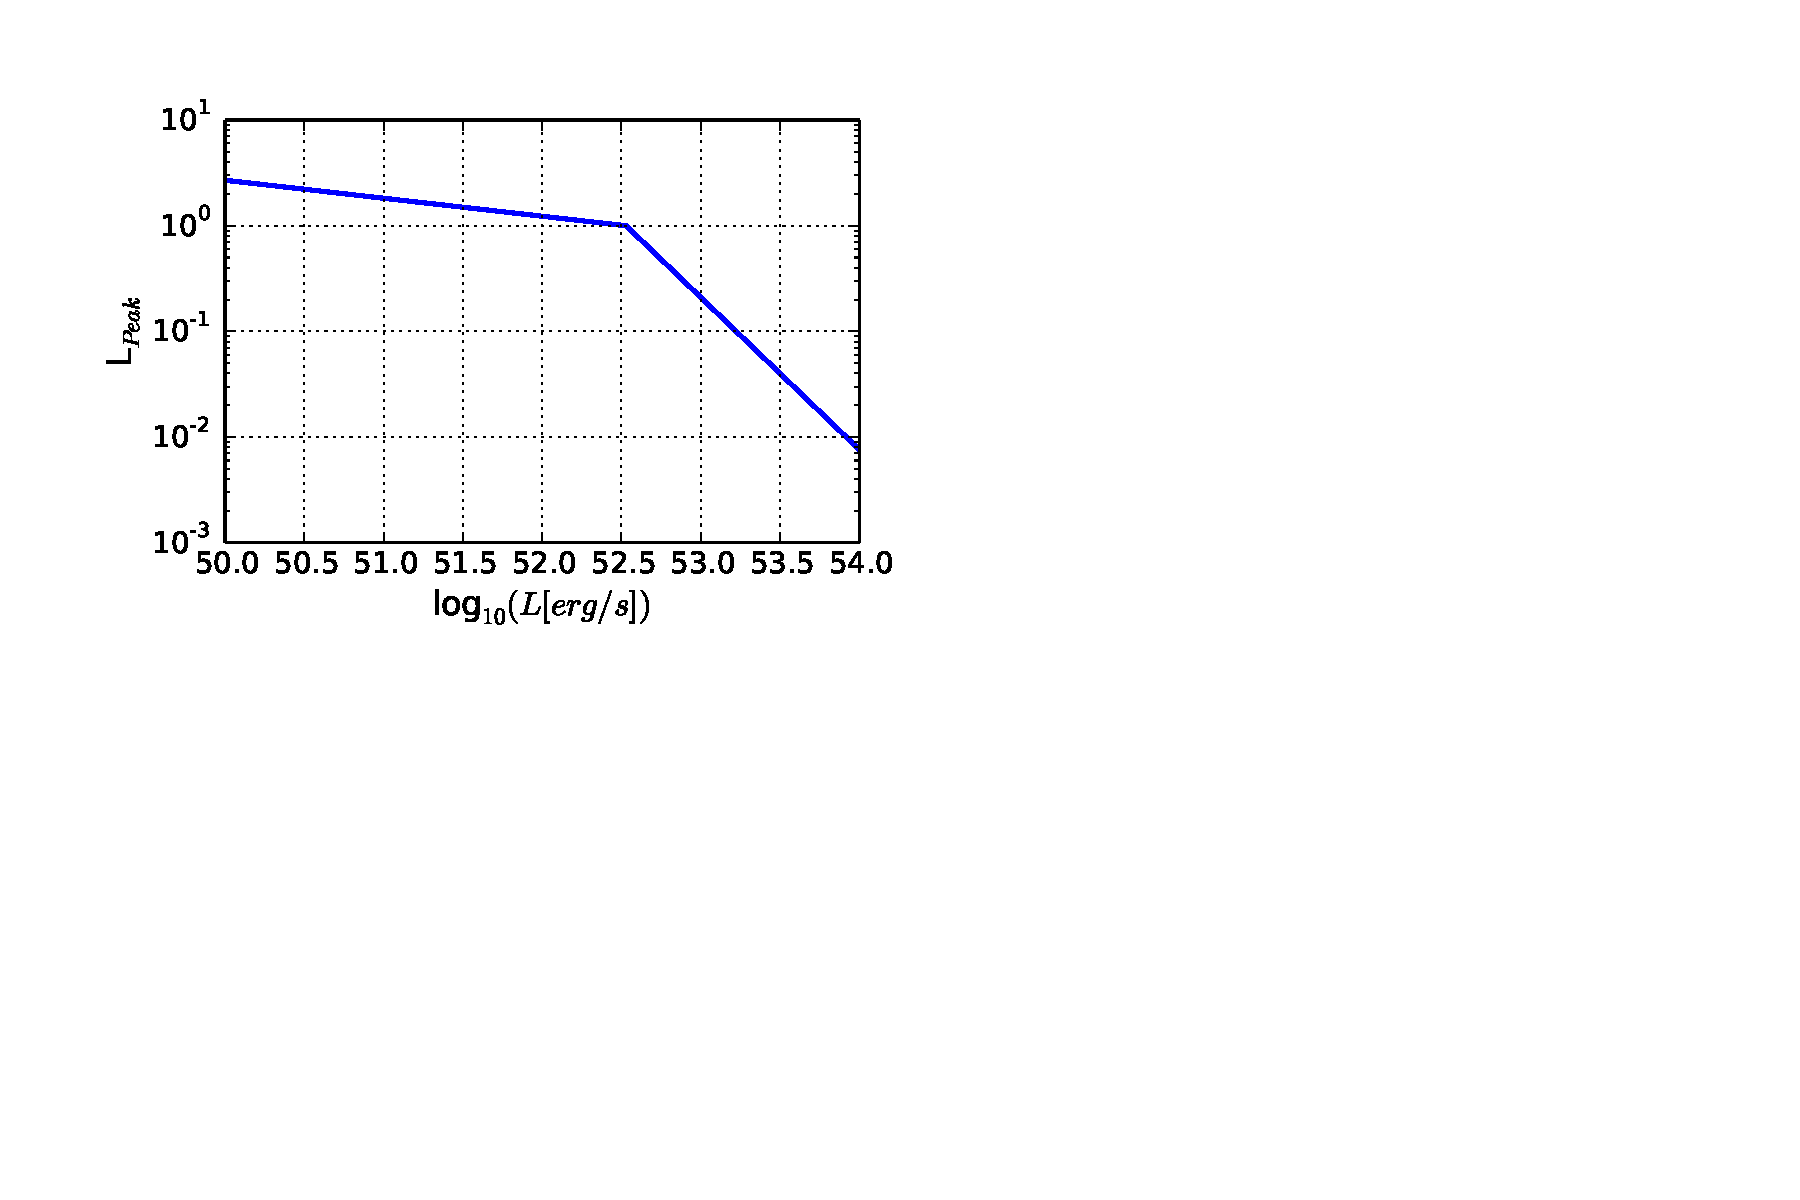
\includegraphics{fig/Lpeak.pdf}
 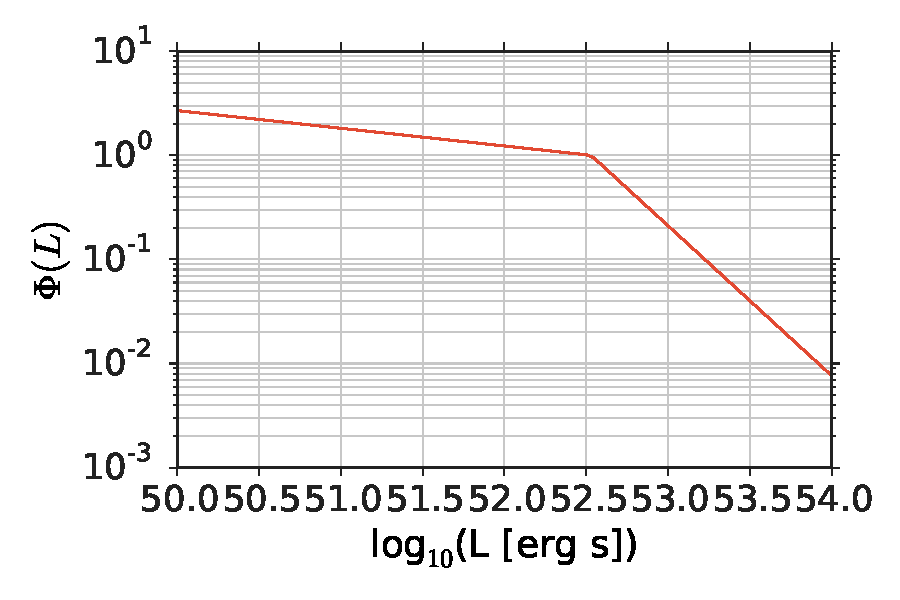
\includegraphics[width=0.6\textwidth]{fig/Lpeak_wp.pdf}
 \caption{The luminosity function derived in the WP model. (deleted this figure 
and use the one including HC?)}
 \label{fig:Lpeak}
% \end{minipage}
\end{figure}